\chapter{Analysis and modeling}
\section{Fixed source}
\subsection{Modal correlation}
\begin{figure}[h]
  \centering
  \begin{tabular}{cc}
  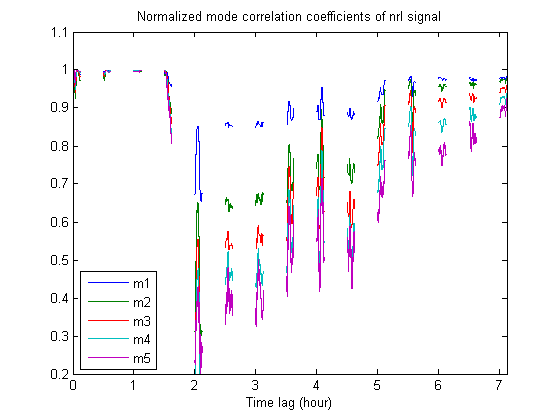
\includegraphics[width=0.5\textwidth]{mode_corr_nrl.png}\\
  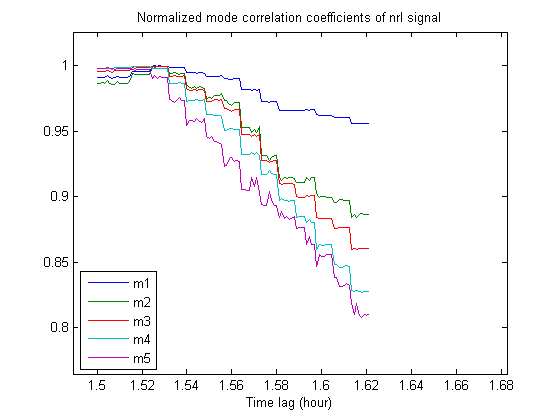
\includegraphics[width=0.5\textwidth]{mode_corr_nrl1.png}
  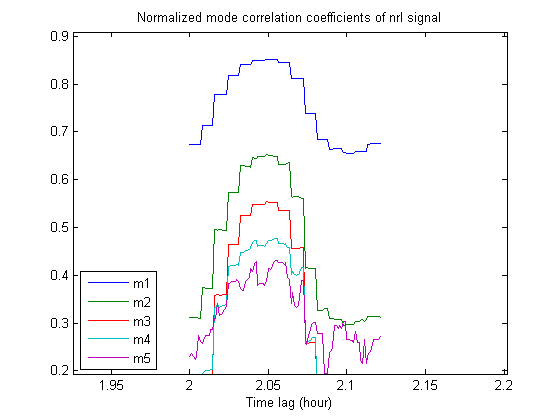
\includegraphics[width=0.5\textwidth]{mode_corr_nrl2.png}
  \end{tabular}
  \caption{Normalized mode correlation coefficients of NRL signal ( reference time = 17-Aug-2006 20:00:00, fc = 300hz) }\label{fig:mc_1}
\end{figure}

Correlation starts to drop after 1.5 hours ( around 21:30). Check the modal decomposition plot above, that's when mode 1,3,4,5 start to break up. From radar image, it can be seen the IW has arrived at the receiver, but has not occupied the entire acoustic track yet. After 2 hours (around 22:00), the correlation drops to the lowest, then slowly bounce back. The lower modes show higher correlation.
\section{Mobile source} \subsection{Modal correlation}
\begin{figure}[h]
  \centering
  \begin{tabular}{cc}
  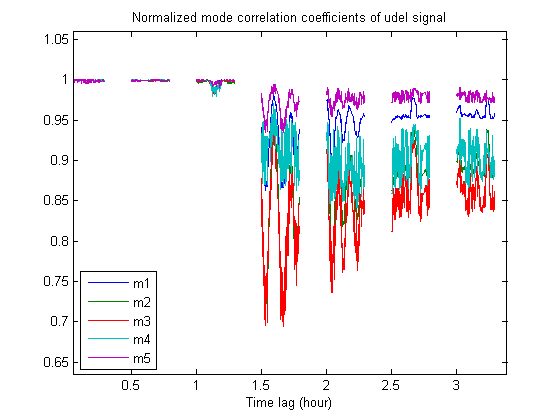
\includegraphics[width=0.5\textwidth]{mode_corr_udel.png}\\
  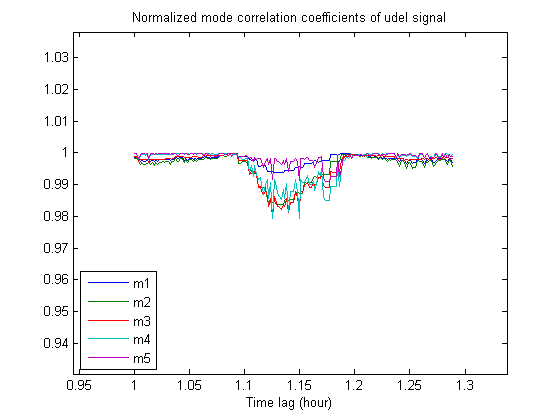
\includegraphics[width=0.5\textwidth]{mode_corr_udel1.png}
  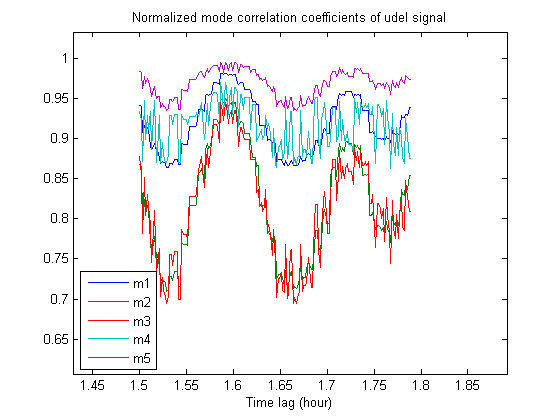
\includegraphics[width=0.5\textwidth]{mode_corr_udel2.png}
  \end{tabular}
  \caption{Normalized mode correlation coefficients of UDEL( R.V. Sharp ) signal ( reference time = 17-Aug-2006 20:10, fc = 150hz).}\label{fig:mc_2}
\end{figure}
Small dip after 1.1 hours ( around 21:20). From radar image, it can be seen a small IW has arrived at the receiver, but the major IW is still 15min away. After 1.5-1.7 hours (around 21:40-21:50), the correlation drops to the lowest, then slowly bounce back. Counterintuitively, the 5th mode shows the highest correlation. The 1st and 4th modes show similar correlation, so do the 2nd and 3rd modes.

\section{PE model}
